
\section{Motivation}

% The motivation for this thesis mainly includes two parts, in the first part, we illustrate the roots of container-based server consolidation problem. In the second parts, we explain the motivations for the objectives.

% \subsection{Motivation For Container-based Server Consolidation Problem}




% Server consolidation \cite{Zhang:2010vo} resolves the low utilization problem by gathering applications or VMs into a fewer number of physical machines (PMs), so that the resource utilization of PMs are maintained at a high level. In the meanwhile, idle servers are turned off to save energy. Traditional server consolidation is VM-based, in comparison with 
% a server host a single application, it can dramatically improve the resource utilization. 


% \begin{figure}
% 	\centering
% 	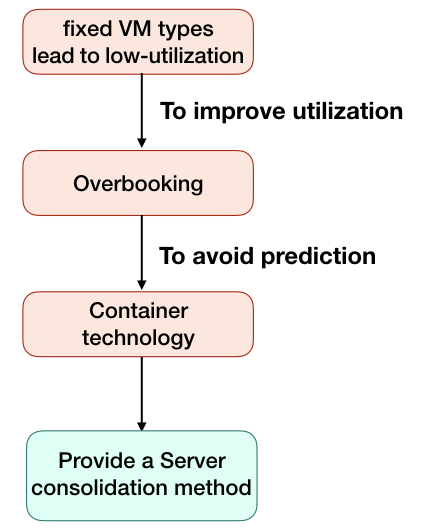
\includegraphics[width=0.3\textwidth]{pics/problem_flow.png}
% 	\caption{The root of container technology}
% 	\label{fig:root}
% \end{figure}
% \begin{enumerate}
% \item Container is a new virtualization technology which provides an operating level of virtualization.
% % Figure \ref{fig:root} illustrates the root of container technology from an energy efficient point of view. 

% In order to solve this problem, overbooking strategy tends to place more VMs than the server's maximum capacity. However, this technique is highly relied on workload prediction on the application running in a VM. Otherwise, servers are easily overloaded. Container technique can improve the utilization by further partitioning VM into resource isolated chunks. Therefore, multiple applications can share the same VM. This technique avoids the prediction of workload as well as improving the utilization. 



% This container technology brings many advantages to current Cloud industry\cite{Felter:2015ki}but it also brings difficulties for server consolidation. Container-based server consolidation adds another level of abstraction which makes it a two-level vector bin-packing problem.
% Therefore, it motivates us to provide \emph{global optimized} resource allocation solution for container-based data centers.

% \end{enumerate}


% \subsection{Motivation For Research objectives}
Cloud data center has a high dynamic nature where it constrantly receives new requests for resource provisioning and releases old current resources. Therefore, a data center needs different strategies to
handle different scenarios. 

In this thesis, we aims at providing a series of approaches to continuously optimize the a joint allocation of VMs and containers. A continuous optimization procedure mainly involves with three stages: initialization, global consolidation, and dynamic consolidation. Different stages have distinctive goals, therefore, they are considered as separated research questions. In addition, a scalability problem of static optimization is considered as an optional objective.

\begin{enumerate}
\item The initialization, \\
At this stage, a set of applications or containers is allocated to a set of empty VMs and these VMs are allocated to a set of PMs. Initalization problem is also refered as placement problem \cite{Jennings:2015ht} which is fundamental for server consolidation problem.
% Previous research  focus on VM-based optimization
This problem is inherently more difficult than previous VM-based consolidation problem, since  container-based consolidation naturely has a two-level structure. Only a few research focus on this problem, Piraghaj \cite{Piraghaj:2016bw} designs a dynamic allocation system. She proposes a two-step procedure; it first allocates containers to VMs and then allocate containers to VMs. Since, these two-level structure interact each other, separate solution certainly leads to a local optima. Therefore, in this thesis, we will solve the problem simutaneously.
% Most importantly, and therefore can not be solved separately. This is the first research that consider server consolidation has a bi-level optimization problem \cite{Wen:1991kt}. 

In this objective, we will establish the fundamental concepts in studying this joint allocation of containers and VMs including new problem models: price and power model, new problem constraints, and optimization objectives. The major challenges for this objective is to design representations and several EC approaches to solve this problem. More specifically, in designing the EC approach, new search mechanisms, operators will be designed and new representations will be proposed to fit the problem. 

% This task is challenging, since a representation can highly affect the performance of consolidation \cite{SoteloFigueroa:2013be}. 

\item Global consolidation, \\
A Global consolidation is conducted to improve the global energy efficiency in a periodical fashion. Data center constantly receives new allocations, releasing of old resources. These operations degrade the compact structure of a data center. Therefore, the data center needs a global optimization to improve the overall energy efficiency.

The challenges are three folds, firstly, similar with initialization problem, the problem has two level of allocations and they interact with each other. Secondly, like VM-based consolidation, Container-based consolidation is considered as a multi-objective problem with minimization of migration cost as well as keeping a good energy efficiency. Thirdly, consolidation is a time-dependent process which means the previous solution affects the current decision. Previous research only consider each consolidation as an independent process. As a consequence, although in one consolidation, the migration is minimized. It may lead to more migration in the future consolidation. We will consider the robustness of consolidation and propose a novel time-aware server consolidation which takes the previous immediate consolidation and the future consolidation into consideration. 

\item Dynamic consolidation,\\
It takes one container and allocates it to VMs. Since the size of container can be dynamically adjusted, when the an application is under-provision or over-provision, the orginal container is halted, resized and re-allocated. Hence, there is a need to allocate this new container in real time. It is also refered as a dynamic placement problem.

To solve a dynamic placement, heuristics and dispatching rules are often used \cite{Sarin:2011fu, Shi:2011ke, Forsman:2015ca, Beloglazov:2012ji}.  In this scenario, a dispatching rule is considered as a function that determines the priorities of PMs that a container can be placed. However, dynamic placement is much complex than bin-packing problem \cite{Mann:2015ua}. Because of its dynamic nature, human designed heuristics are ill-equipped in approximating solutions when the environment has changed \cite{SoteloFigueroa:2013be}. Multi-objective genetic algorithm (GA) \cite{Xu:2010vh} has been applied. However, GA is too slow for dynamic problem. 

We intend to develop a hyper-heuristic method - Genetic Programming (GP) technique \cite{Banzhaf:1998wc} or artificial immune system \cite{Hofmeyr:2000ju}- to learn from the best previous allocation and automatic evolves dispatching rules to solve this problem. GP has been applied in generating dispatching rules for bin-packing problem \cite{Burke:2006ei, SoteloFigueroa:2013be} and other scheduling problems \cite{Nguyen:2014eu}. The results have shown promising results.

There are mainly two challenges, first, it is difficult to identify the related factors that construct the heuristic. Factors or features are the building blocks of heuristics. It is a difficult task because the relationship between a good heuristic and features are not obvious. Second, representations provide different patterns to construct dispatching rules. It is also unclear what representation is the most suitable for the consolidation problem. 


% and representations must be proposed to capture the characteristic of the joint allocation. 
% 	and the VMs are allocated to physical machines in the second step. Because of the complexity, previous research
% 	only considers the first step. They map the incoming tasks into predefined categories and based on the characteristic of the categories, the size of new virtual machines' resources are decided. After each tasks have chosen its VM type, they are allocated to virtual machines using a lightweight heursitic algorithm. 
% 	We intend to apply an EC-based approach to solve this problem by proposing a coevolutionary that simuetiously decide the virtual machine type as well as the allocation of VMs.


\item Large-scale of static server consolidation problem, \\
	In this case, initialization and global consolidation are belonged to this category, since they are usually conducted in an off-line fashion. 
	Since Cloud data center typically has hundreds of thousands PMs and more, static server consolidation is always very challenging. Many approaches have been proposed in the literature to resolve the problem. There are mainly two ways, both rely on distributed methods, hierarchical-based \cite{Jung:2010dt, Moens:2011gk} and agent-based management systems \cite{Yazir:2010bk}.
	The major problem in agent-based systems is that agents rely on heavy communication to maintain a high-level utilization. Therefore, it causes heavy load in the networking. 
	Hierarchical-based approaches are the predominate methods. In essence, these approaches are centralized methods where all the states of machines within its region are collected and analyzed. The major disadvantage of hierarchical-based approaches is that it only provides local solutions. In fact, it is infeasible and unnecessary to check all the states of machines since the search space is too large and most machines do not need a change. This idea
	motivates a way to improving the effectiveness is to reduce the number of variables so that the search space is narrowed. In this thesis, we are going to investigate the way to eliminate the redundant information.
\end{enumerate}



% Traditional Cloud computing offers three services models: Infrastructure as a Service (IaaS), Platform as a Service (PaaS) and Software as a Service (SaaS). Both IaaS and PaaS describe how does a service provider use the cloud resources. The main difference of these two models are  
% IaaS allows service providers to manage the low-level details including the operating system and libraries. While, PaaS provides a higher level of abstraction where users only focus on the application development without caring the underlying operating system and system-level of resources such as CPU cores and memories. However, one drawback of PaaS is that cloud users must make sure their applications are complete compatible with the platform. And in many of the cases, it is not the situation. In order to solve this problem, a container-based virtualization technology starts to reform the Cloud industry. Container as a Service (CaaS) 
% is a new concept but it has been used in industry for many years. Containers provide an operating system-level of isolation environment for applications. It does not need a hypervisor but complete rely on the operating system. 


% This exciting new technology has bring so many advantages for both Cloud users and Cloud providers. From the providers' perspective, In a large system, running VMs means there are probably many same operating systems occupying memories and storages. Lightweight containers share operating system and therefore, there are more rooms for softwares. It increases the capability of Cloud data centers. Furthermore, in terms of resource utilization, it provides much finer granularity operation than a VM-based Cloud model. Containers partition
% a VM into smaller chunks so that with appropriate management, better energy efficiency can be achieved. From the cloud users' perspective, each container provides separated libraries for specific application.  Therefore, it does not contrained by the underlying platform. Like PaaS, Cloud users do not need to concern the scalability of applications. 
% Therefore, CaaS can potentially become one of the main stream in the future Cloud computing industry. 

% Secondly, energy-efficent computing has been the major concern since the begining of computers. Specifially, Cloud computing has become a popular form. Large-scale data centers have been built around the world. A data center can consume huge amount of energies and it needs to improve its energy-efficiency from multiple perspectives. As we discussed in the Introduction, computing servers are one of the major contribution to the energy consumption. 
% And according to observation by \cite{}, the average utilization resource are still very low which causes huge energy wastage. As we mentioned above, the container technolgy provides a better way of managing resources, it has the potential to largly improve the utilization than current VM-based Cloud model because it avoids some of the major drawbacks of VM-based model. 

% Thirdly, because the container technology is relatively new, previous research are mostly focus on IaaS model and so that the server consolidation has based on the VM-level. However,   

% Frist is this new technology of container that can potentially change the landscape of
% Cloud computing. It has so many benefits but also it brings difficulty in managing resources.

% Second, from green computing point of view, we still need to manage resource so that, the 
% data centers consume less energy. And container technolgy actually bring a better chance to
% be more energy-efficient than previous VM based technology.
% Third, it is very difficult to manage this container-based resources because of the problem-nature is too complicated. And existed algorithms can not be directly applied on it.
% Fourth, the evolutioanry computation provides a good framework to handle such difficult problem.

% \textcolor{Blue}{Motivation is what is now lack from the literature.} \\

% The advantage of Platform as a Service (PaaS) has been discovered in the recent years. 
% The disadvantage of tranditional IaaS model has been discovered in the recent years \cite{Mann:2016hx}.
% In IaaS, on one hand, cloud customers need to manage the low-level details ranging from application capacity estimation,
% resource planning and selection and deployment. 
% On the other hand, Cloud providers manage resource provisioning and allocation. 
% Although these two tasks are seemingly different, 


% The container as a Service (CaaS) cloud model has gain increasing attention in the recent years.
% However, the energy efficiency in CaaS cloud environment has not been investigate. 
% Particularly, the virtual machine and container joint consolidation is the core problem.
% Therefore, in this thesis, we will focus on the end-to-end energy-aware server consolidation on container-based
% Cloud. In the meanwhile,  a major research direction of large scale server consolidation is also considered. 
% The end-to-end server consolidation refers to the server consolidation techniques used
% in the different stages throughout the routine Cloud resource management including  initial VM provisioning and placement, dynamic VM placement, and static VM placement:
